\begin{document}
The BJT operates similarly to the NMOS circuit. The difference being it is now an NPN transistor and is therefore a current controlled voltage source, as opposed to the NMOS which is a voltage controlled. The values for the BJT circuit were not solved for, but instead provided as part of the lab, which can be seen in Table \ref{tab:bjttab}

\begin{table}[H]
	\centering
	\caption{BJT experimental values}
	\label{tab:bjttab}
	\begin{tabular}{|c|c|} \hline
		$Q_1, Q_2, Q_3$ & 2N3904        \\ \hline
		$R_ref$         & 19.3k$\Omega$ \\ \hline
		$R_C$           & 4.7k$\Omega$  \\ \hline
		$R_B$           & 10k$\Omega$   \\ \hline
		$R_E$           & 3.3k$\Omega$  \\ \hline
		$R_L$           & 1k$\Omega$    \\ \hline
		$C_B$, $C_C$, $C_E$ & 500nF      \\   \hline
		Gain            & 30db          \\  \hline
		Lower cutoff    & 3 kHz         \\  \hline
		Upper cutoff    & 100 MHz       \\  \hline  
	\end{tabular}
\end{table}
 The simulated circuit is shown in Figure \ref{fig:bjtsimcir}.
 
 \begin{figure}[H]
 	\centering
 	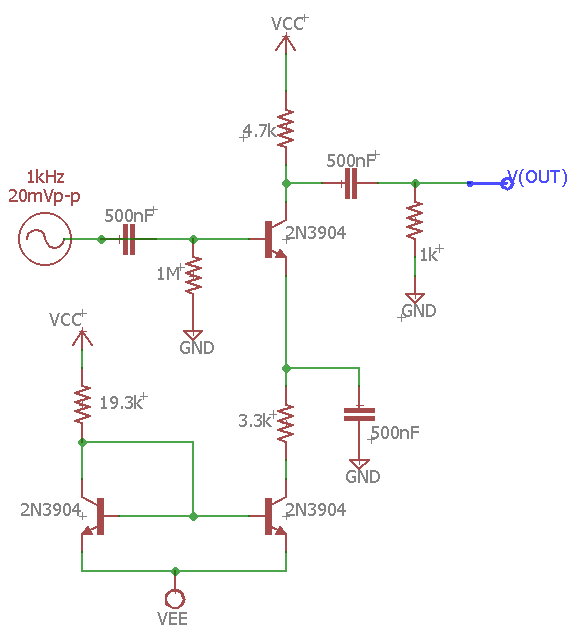
\includegraphics[width=.55\textwidth]{CircuitDevelopment/BJT_sim.png}
 	\caption{Simulated circuit of BJT}
 	\label{fig:bjtsimcir}
 \end{figure}
 
 
 The simulations of the BJT follow and were performed in Matlab integrated with NGspice. The frequency response of the circuit can be seen in Figure \ref{fig:bjtsimfreq}. 

\begin{figure}[H]
	\centering
	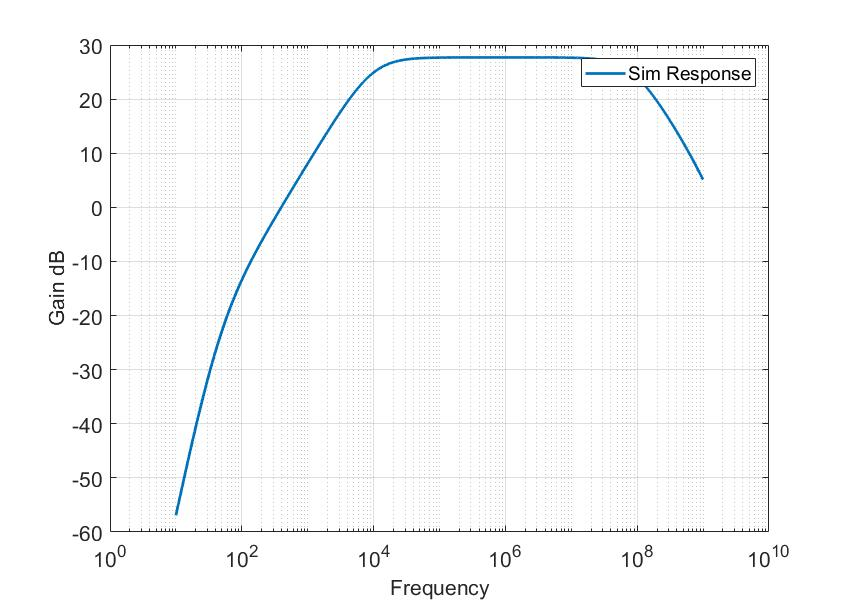
\includegraphics[width=.55\textwidth]{CircuitDevelopment/BJT_bandwidth.jpg}
	\caption{Simulated frequency response of BJT}
	\label{fig:bjtsimfreq}
\end{figure}

Notably, the 3dB lower cutoff is greater than 1 kHz. The corresponding passband gain is significantly higher than 20 dB. This is not ideal, because the output could begin to saturate due to excessive gain. The FFT of the BJT can be seen in Figure \ref{fig:bjtFFT}

\begin{figure}[H]
	\centering
	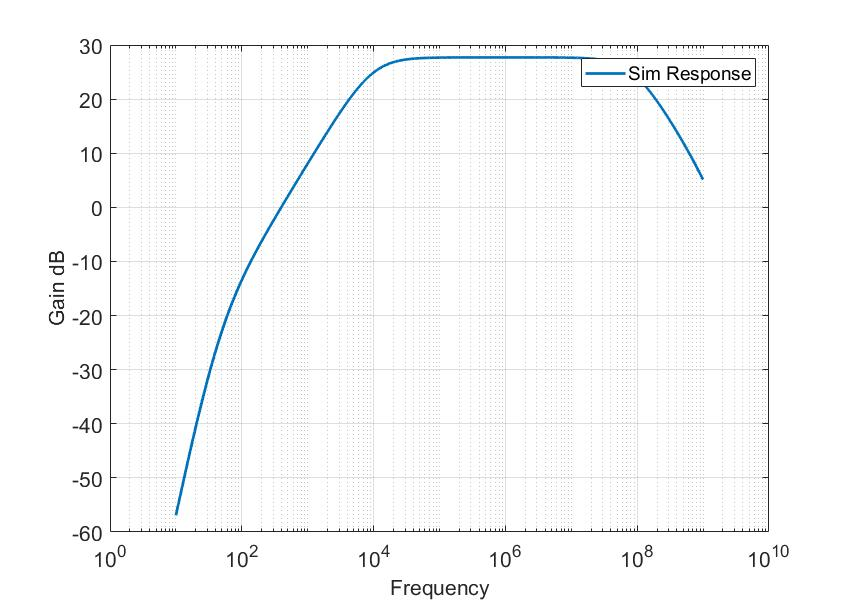
\includegraphics[width=.55\textwidth]{CircuitDevelopment/BJT_bandwidth.jpg}
	\caption{Simulated FFT BJT circuit}
	\label{fig:bjtFFT}
\end{figure}

The BJT achieved a far smaller second harmonic distortion than the NMOS, with only a .25\% distortion for the 2 kHz harmonic.



 



\end{document}